\chapter{Fine-Tuning for Production --- A SWE's Playbook}
\label{ch:finetuning}

\begin{quote}
\itshape
``Don't fine-tune until you've exhausted prompting. Don't train from scratch until you've exhausted fine-tuning.''\\
--- Common wisdom in ML engineering
\end{quote}

\vspace{0.5cm}

\noindent
Fine-tuning is the process of adapting a pre-trained (and typically post-trained) model to a specific task, domain, or behavior. For software engineers, fine-tuning occupies a critical middle ground in the build-vs-buy decision: it's more powerful than prompt engineering but far less expensive than training a model from scratch.

This chapter provides a practical playbook for fine-tuning in production environments. We cover when to fine-tune (and when not to), the modern parameter-efficient techniques that make fine-tuning accessible, the data preparation and evaluation practices that determine success or failure, and the deployment strategies that get fine-tuned models into production reliably.

\section{The Decision Framework: When to Fine-Tune}

Before investing in fine-tuning, engineers should systematically evaluate simpler alternatives. Fine-tuning is powerful but costly---in engineering time, compute, and ongoing maintenance. The decision tree in Figure~\ref{fig:finetune-decision} provides a structured approach.

\begin{figure}[htbp]
\centering
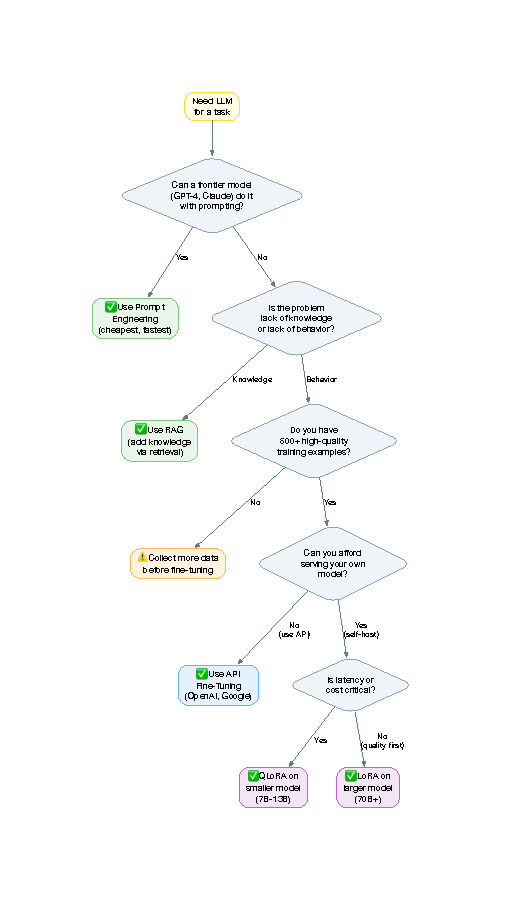
\includegraphics[width=\textwidth]{diagrams/compiled/ch04/finetune-decision.pdf}
\caption{Decision framework: when to fine-tune vs. alternative approaches}
\label{fig:finetune-decision}
\end{figure}

\subsection{Start with Prompt Engineering}

Prompt engineering is always the first thing to try. It requires no training infrastructure, no dataset curation, and changes can be deployed in minutes. Modern frontier models respond well to:

\begin{itemize}[leftmargin=*]
    \item \textbf{System prompts}: Detailed behavioral instructions
    \item \textbf{Few-shot examples}: 3--10 input-output examples in the prompt
    \item \textbf{Chain-of-thought}: Instructing the model to reason step by step
    \item \textbf{Structured output}: Requesting JSON, XML, or other structured formats
\end{itemize}

\begin{tipbox}[When Prompting Is Enough]
If your task can be described clearly in natural language with a few examples, and a frontier model (GPT-5.5, Claude Opus 4.8, Gemini Pro 3.1) achieves acceptable quality, \emph{don't fine-tune}. Instead, invest in prompt testing, versioning, and evaluation infrastructure.
\end{tipbox}

\subsection{Consider RAG Before Fine-Tuning}

Retrieval-Augmented Generation (RAG) is often confused with fine-tuning but serves a different purpose:

\begin{itemize}[leftmargin=*]
    \item \textbf{Fine-tuning} changes the model's \emph{behavior} and \emph{style}: how it formats responses, what tone it uses, what reasoning patterns it follows
    \item \textbf{RAG} changes the model's \emph{knowledge}: what facts and information it has access to
\end{itemize}

If your problem is ``the model doesn't know about our internal documentation,'' RAG is the answer, not fine-tuning. If your problem is ``the model's responses don't match our company's tone and format requirements,'' fine-tuning is more appropriate.

\subsection{When Fine-Tuning Is the Right Choice}

Fine-tune when:

\begin{enumerate}[leftmargin=*]
    \item \textbf{Style and format}: You need consistent output in a specific format that few-shot prompting can't reliably achieve
    \item \textbf{Latency}: You need a smaller, faster model that matches a larger model's quality on your specific task
    \item \textbf{Cost}: You're making millions of API calls and a smaller fine-tuned model would significantly reduce cost
    \item \textbf{Domain specialization}: Your domain has specialized vocabulary or reasoning patterns (legal, medical, financial) that benefit from domain-specific training
    \item \textbf{Behavioral consistency}: You need the model to reliably follow complex behavioral guidelines that are too long or nuanced for a system prompt
    \item \textbf{Privacy}: You can't send data to third-party APIs and need an on-premise model
\end{enumerate}

\section{Parameter-Efficient Fine-Tuning (PEFT)}

Full fine-tuning---updating all of a model's parameters---is prohibitively expensive for most teams. A 70B parameter model requires hundreds of gigabytes of GPU memory for optimizer states alone. \term{Parameter-efficient fine-tuning} (PEFT) methods solve this by updating only a small number of parameters while keeping the rest frozen.

\subsection{LoRA: Low-Rank Adaptation}

\term{LoRA}~\cite{hu2022lora} is the most widely used PEFT method. The key insight: the weight updates during fine-tuning tend to be low-rank---they can be approximated as the product of two small matrices.

Instead of updating a weight matrix $W \in \mathbb{R}^{d \times d}$, LoRA adds a low-rank decomposition:

$$W' = W + BA$$

where $B \in \mathbb{R}^{d \times r}$ and $A \in \mathbb{R}^{r \times d}$, and $r \ll d$ (typically $r = 8$ to $64$).

\begin{figure}[htbp]
\centering
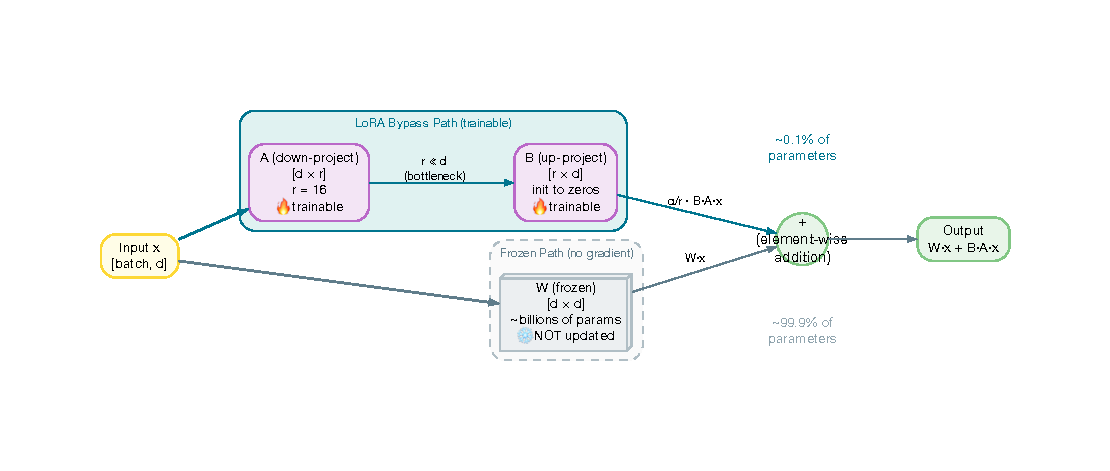
\includegraphics[width=\textwidth]{diagrams/compiled/ch04/lora-architecture.pdf}
\caption{LoRA architecture: the frozen base weights $W$ are bypassed by a low-rank decomposition $BA$, where only $A$ and $B$ are trained}
\label{fig:lora-architecture}
\end{figure}


\begin{lstlisting}[language=Python, caption={LoRA implementation (simplified)}]
import torch
import torch.nn as nn

class LoRALayer(nn.Module):
    """Low-Rank Adaptation layer."""
    
    def __init__(self, 
                 original_layer: nn.Linear, 
                 rank: int = 16,
                 alpha: float = 32.0):
        super().__init__()
        self.original = original_layer
        self.original.weight.requires_grad = False  # Freeze
        
        d_in = original_layer.in_features
        d_out = original_layer.out_features
        
        # Low-rank matrices
        self.lora_A = nn.Parameter(
            torch.randn(d_in, rank) * 0.01
        )
        self.lora_B = nn.Parameter(
            torch.zeros(rank, d_out)  # Initialize B to zero
        )
        self.scaling = alpha / rank
    
    def forward(self, x: torch.Tensor) -> torch.Tensor:
        # Original output + low-rank update
        original_out = self.original(x)
        lora_out = (x @ self.lora_A @ self.lora_B) * self.scaling
        return original_out + lora_out
\end{lstlisting}

The benefits are dramatic:

\begin{table}[htbp]
\centering
\caption{Memory requirements: full fine-tuning vs. LoRA}
\label{tab:lora-memory}
\begin{tabularx}{\textwidth}{lrrX}
\toprule
\textbf{Model} & \textbf{Full FT Memory} & \textbf{LoRA (r=16)} & \textbf{Trainable Params (\%)} \\
\midrule
LLaMA 7B   & $\sim$56 GB   & $\sim$16 GB  & 0.1\% \\
LLaMA 13B  & $\sim$104 GB  & $\sim$28 GB  & 0.08\% \\
LLaMA 70B  & $\sim$560 GB  & $\sim$160 GB & 0.04\% \\
\bottomrule
\end{tabularx}
\end{table}

\subsection{QLoRA: Quantized LoRA}

\term{QLoRA} combines LoRA with model quantization to further reduce memory. The base model weights are loaded in 4-bit precision (using the NF4 quantization format), while the LoRA adapters are trained in 16-bit. This allows fine-tuning a 70B model on a single 48GB GPU---a capability that has democratized fine-tuning.

\begin{lstlisting}[language=Python, caption={QLoRA training setup with Hugging Face}]
from transformers import AutoModelForCausalLM, BitsAndBytesConfig
from peft import LoraConfig, get_peft_model

# 4-bit quantization config
bnb_config = BitsAndBytesConfig(
    load_in_4bit=True,
    bnb_4bit_quant_type="nf4",
    bnb_4bit_compute_dtype=torch.bfloat16,
    bnb_4bit_use_double_quant=True,
)

# Load quantized model
model = AutoModelForCausalLM.from_pretrained(
    "meta-llama/Llama-3.1-8B-Instruct",
    quantization_config=bnb_config,
    device_map="auto",
)

# Add LoRA adapters
lora_config = LoraConfig(
    r=16,                      # Rank
    lora_alpha=32,             # Scaling factor
    target_modules=[           # Which layers to adapt
        "q_proj", "k_proj", "v_proj", "o_proj",
        "gate_proj", "up_proj", "down_proj",
    ],
    lora_dropout=0.05,
    bias="none",
    task_type="CAUSAL_LM",
)

model = get_peft_model(model, lora_config)
model.print_trainable_parameters()
# Output: trainable params: 13,107,200 || all params: 8,043,839,488
#         || trainable%: 0.163%
\end{lstlisting}

\section{Dataset Preparation}
\label{sec:dataset-prep}

The most common cause of fine-tuning failure is not the training process---it's the dataset. Software engineers accustomed to clean, structured data are often surprised by how much effort goes into curating a fine-tuning dataset.

\subsection{Quality Over Quantity}

The cardinal rule: \textbf{500 excellent examples beat 50,000 mediocre ones}. Each training example teaches the model a pattern. If your examples contain errors, inconsistencies, or low-quality outputs, the model will faithfully learn those patterns.

Dataset quality checks that every example must pass:

\begin{itemize}[leftmargin=*]
    \item \textbf{Structural}: Last message must be from assistant. No empty messages. All code blocks matched and closed.
    \item \textbf{Content}: No refusal patterns (``As an AI,'' ``I cannot'') in training data---these teach the model to refuse. Response length within expected bounds (too short = low effort, too long = padding).
    \item \textbf{Consistency}: All examples follow the same output format. If 80\% use bullet points and 20\% use paragraphs, the model will randomly switch between them.
    \item \textbf{Diversity}: Balanced across categories. If 90\% of examples are billing queries, the model will try to make everything about billing.
\end{itemize}

\subsection{Data Formatting}

All modern fine-tuning uses the \emph{chat format}---a structured sequence of system, user, and assistant messages with model-specific special tokens. The Hugging Face \code{tokenizer.apply\_chat\_template()} method handles this automatically for all major model families (Llama 4, Mistral, Gemma, etc.). Never format chat templates manually---use the tokenizer's built-in template to avoid subtle encoding bugs.

\section{Evaluation-Driven Development}
\label{sec:eval-driven}

The most important lesson from production fine-tuning: \textbf{define your evaluation metrics before you start training}. Without clear metrics, you have no way to know if your fine-tuned model is better than the base model, or if changes to your dataset or hyperparameters actually help.

\subsection{Building an Evaluation Suite}

A fine-tuning evaluation suite should measure three dimensions: \textbf{format compliance} (does the output match the expected schema?), \textbf{accuracy} (does it match the reference answer?), and \textbf{relevance} (is the content actually useful?). Run this suite against four baselines: the base model zero-shot, the base model few-shot, any previous fine-tuned version, and the current candidate. The fine-tuned model must beat \emph{all four} to be promoted---if few-shot prompting matches the fine-tuned model's quality, the fine-tuning investment isn't justified.

\section{Deployment: Getting Fine-Tuned Models to Production}
\label{sec:deployment}

A fine-tuned model is useless if it can't be deployed reliably. This section covers the practical aspects of model deployment, from quantization to serving infrastructure.

\subsection{Quantization for Inference}

Fine-tuned models are typically quantized before deployment to reduce memory and increase throughput. The most common quantization formats:

\begin{itemize}[leftmargin=*]
    \item \textbf{GPTQ}: Post-training quantization using second-order information. Produces 4-bit models with minimal quality loss. Requires a calibration dataset.
    \item \textbf{AWQ}: Activation-aware weight quantization. Preserves salient weights that are important for accuracy. Often slightly better quality than GPTQ.
    \item \textbf{GGUF}: Quantization format used by llama.cpp for CPU inference. Supports various bit widths (Q4\_K\_M, Q5\_K\_M, Q8\_0). Excellent for edge deployment.
\end{itemize}

\subsection{Model Serving}

For production serving, the two leading options are:

\begin{itemize}[leftmargin=*]
    \item \textbf{vLLM}: PagedAttention-based serving engine with excellent throughput. Supports continuous batching, tensor parallelism, and LoRA adapter hot-swapping.
    \item \textbf{TensorRT-LLM}: NVIDIA's optimized inference engine. Best performance on NVIDIA GPUs but more complex to set up.
\end{itemize}

A critical production capability: \textbf{LoRA adapter hot-swapping}. Both vLLM and TensorRT-LLM support loading multiple LoRA adapters on a single base model, routing requests to different adapters at inference time. This means you can serve dozens of specialized fine-tuned models (one per customer, one per domain) without multiplying your GPU costs.

Figure~\ref{fig:finetune-pipeline} summarizes the complete fine-tuning pipeline from dataset preparation through production deployment.

\begin{figure}[htbp]
\centering
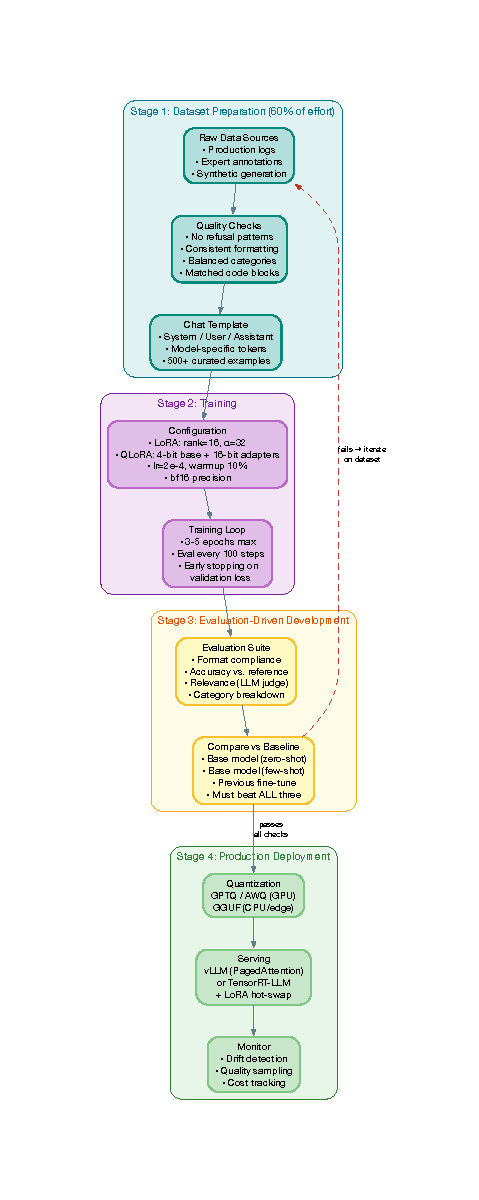
\includegraphics[width=\textwidth]{diagrams/compiled/ch04/finetune-pipeline.pdf}
\caption{End-to-end fine-tuning pipeline: 60\% of effort goes into dataset preparation. The evaluation stage gates promotion---the fine-tuned model must beat all baselines. Failure feeds back to dataset iteration.}
\label{fig:finetune-pipeline}
\end{figure}

\begin{keytakeaway}
Fine-tuning is a powerful technique, but it's not a shortcut. The effort required to curate high-quality datasets, build evaluation infrastructure, and maintain fine-tuned models in production is substantial. Only fine-tune when simpler approaches (prompting, RAG) are demonstrably insufficient for your use case.
\end{keytakeaway}

\section{Case Study: Fine-Tuning for Enterprise Code Generation}

A mid-size enterprise (500 engineers, 200+ internal repositories) wanted to build a code completion tool that understood their internal frameworks, coding conventions, and API patterns. Here's how they approached it:

\begin{casestudy}[Enterprise Code Generation]
\textbf{Problem}: GitHub Copilot suggestions didn't understand the company's internal framework APIs, style guidelines, or architectural patterns.

\textbf{Approach}:
\begin{enumerate}
    \item Collected 15,000 high-quality code completions from their top engineers' commit history
    \item Filtered for code that passed all linting rules and had been approved in code review
    \item Fine-tuned LLaMA 3 8B using QLoRA (rank=32) for 3 epochs
    \item Built an A/B testing framework to compare against Copilot
\end{enumerate}

\textbf{Results}:
\begin{itemize}
    \item 40\% higher acceptance rate for completions involving internal APIs
    \item 15\% higher acceptance rate overall
    \item Inference cost: \$0.002 per completion vs. \$0.01 for Copilot
    \item Total project cost: \$5,000 in compute + 3 weeks of engineering time
\end{itemize}

\textbf{Key lesson}: The dataset quality was more important than the model size. They initially tried a 70B model with a hastily assembled dataset and got worse results than the 8B model trained on carefully curated data.
\end{casestudy}

\section{Chapter Summary}

Fine-tuning is a core capability in the AI engineer's toolkit. The key takeaways:

\begin{enumerate}[leftmargin=*]
    \item \textbf{Follow the decision tree}: Prompting $\rightarrow$ RAG $\rightarrow$ fine-tuning $\rightarrow$ pre-training. Each step is 10x more expensive than the last.
    \item \textbf{LoRA/QLoRA are game-changers}: They reduce the cost and complexity of fine-tuning by 10--100x compared to full fine-tuning.
    \item \textbf{Data quality is everything}: 500 perfect examples beat 50,000 mediocre ones.
    \item \textbf{Evaluate before, during, and after}: Build your eval suite first, then use it to guide every decision.
    \item \textbf{Plan for deployment}: Quantization, serving infrastructure, and adapter management are not afterthoughts.
\end{enumerate}
